\chapter{Carbon: Cloud Workspaces}
\label{chap:carbon}

\section{Purpose}
The purpose of this chapter is to introduce Carbon, a web application for allows users to create personal online modeling and simulation environments.
Carbon may be used by modelers to produce and collaborate new models online, or easily reproduce results from a publication.
While Carbon is still under rapid development, many core features are already in place, which will be discussed here.

\section{Motivation}

For science to advance, experimental reproducibility is crucial. 
For computational experiments, in theory, a script or program could describe every step taken by the computer, which provides even greater detail than the analogous non-computational experimental descriptions published in journals.
However, the reality is that sometimes the code is not available, either unpublished or nonexistent when the interactive software system does not track the users’ actions.
Even if the researcher shares code, it may require specific versions of software platforms and packages, which may be difficult to acquire.

While this problem likely will require a combined effort of different measures, one approach is to move researchers towards software platforms and practices that encourage transparency and reproducibility.

\section{Solution}

Carbon aims to lower the barrier to obtaining bio-modeling software by providing personal computing environments available through the browser.
Each researcher can register and log in to access a suite of scientific apps (Figure~\ref{Figure:carbon-login}).
Currently, the two apps that are included are a model visualization and file management tool called Workspaces (developed by this author with Graphene), and IPython Notebook \autocite{perez2007ipython}.

In Workspaces (Figure~\ref{Figure:carbon-workspaces}), the user can perform a variety of file system manage actions, such as creating new folders and files, either through upload or copy-and-paste.
All files within the workspace may be viewed and manipulated through a text editor (Figure~\ref{Figures:carbon-workspaces-files}).
Model file formats, such as SBML, will also be accompanied with a layout view (Figure~\ref{Figure:carbon-workspaces-model-view}).

\subsection{Python environment for model exploration, analysis, and curation}

Workspaces is also provides integration with IPython Notebooks.
A model file may be easily converted converted into a notebook file (Figure~\ref{Figure:carbon-workspace-convert-to-ipython}).
By default, the new notebook filename is based off the original model file.

The newly created notebook is detected immediately by IPython Notebook (Figure~\ref{Figure:carbon-workspace-ipython-view}), as IPython Notebook and Workspaces share the same working directory.
Within the notebook, helper scripts and functions have already been generated that can be immediately executed to the load and run a simulation of the source model (Figure~\ref{Figure:carbon-ipython-template}).
In addition, a pre-build interactive simulation widget is built for the loaded model (Figure~\ref{Figure:carbon-ipython-widget}).
Sliders are created for each kinetic parameter within the model, and upon sliding, the simulation graph is updated with the new values.
Input boxes are also available for changing start and end simulation times and the number of steps.

A number of python libraries are already installed inside the workspace, including Tellurium, PySCeS, and Pandas.
Users may also install any additional libraries that they may need, either through the terminal or using a package manager such as \texttt{pip}, without affecting the environment of other users.

A plugin has also been developed which allows users to generate URL links from Combine Archive files that upon opens to a portal page to allow the user to open the entire model project on Carbon or locally if they have the necessary software installed (Figure~\ref{Figure:carbon-combine-archive}).

\autocite{ragan2013collaborative}

\section{Implementation}

Carbon uses two top level processes a node.js server and a MongoDB database (Docker is also used extensively, which will be discussed in section~\ref{sec:docker}).
Node.js was selected as the platform because of its high performance and ability to use JavaScript on the server \autocite{tilkov2010node}, which eases development by keeping the same programming language between server and client.
Carbon also uses the node.js package management system, \texttt{npm}, extensively to management software dependencies and to easily deploy on multiple platforms. \autocite{lerner2011forge}




\subsection{Database}

\subsubsection{Express.js and Flask}
\subsubsection{MongoDB}
\subsection{Workspace isolation}
\label{sec:docker}
\subsubsection{Linux containers}
\subsubsection{Services and ports}
\subsection{Asynchronous programming}
\subsubsection{Highly nested callbacks}
\subsubsection{Use of promises}
\subsection{Conversion of model formats to IPython notebooks}

\section{Future Directions}
\subsection{Security}

\begin{figure}
  \centering
  \includegraphics[width=\textwidth, page=28, trim=0cm 0cm 12cm 0cm, clip=true]{images/Figures.pdf}
  \caption{Architecture of Carbon.}
  \label{fig:carbon-architecture}
\end{figure}


\begin{figure}
  \centering
  \begin{subfigure}[b]{\textwidth}
    \includegraphics[width=\textwidth, page=9, trim=0.37cm 3.65cm 13.1cm 3.3cm, clip=true]{images/Figures.pdf}
    \caption{The Carbon landing page.}
    \label{Figure:carbon-login-landing}
  \end{subfigure}
  \begin{subfigure}[b]{\textwidth}
    \includegraphics[width=\textwidth, page=9, trim=13.1cm 3.65cm 0.37cm 3.3cm, clip=true]{images/Figures.pdf}
    \caption{Once the user is logged in, the navigation bar will populate with available applications.}
    \label{Figure:carbon-login-logged-in}
  \end{subfigure}
  \caption{Carbon provides a user-specific workspaces.}
  \label{Figure:carbon-login}
\end{figure}

\begin{figure}
  \centering
  \begin{subfigure}[b]{\textwidth}
    \includegraphics[width=\textwidth,page=10,trim=0.37cm 3.65cm 13.1cm 3.3cm, clip=true]{images/Figures.pdf}
    \caption{The left sidebar contains a collapsible directory tree view.
      Each directory also contains expandable option buttons for file creation, upload, and deletion.}
    \label{Figure:carbon-workspaces-view}
  \end{subfigure}
  \begin{subfigure}[b]{\textwidth}
    \includegraphics[width=\textwidth,page=10,trim=13.1cm 3.65cm 0.37cm 3.3cm, clip=true]{images/Figures.pdf}
    \caption{New folders can also be created anywhere within the directory tree.}
    \label{Figure:carbon-workspaces-new-folder}
  \end{subfigure}
  \caption{Workspace app is a plugin to Carbon that allows easy file management and browsing of model files.}
  \label{Figure:carbon-workspaces}
\end{figure}

\begin{figure}
  \centering
  \begin{subfigure}[b]{\textwidth}
    \includegraphics[width=\textwidth,page=11,trim=0.37cm 3.65cm 13.1cm 3.3cm, clip=true]{images/Figures.pdf}
    \caption{Users may create new files in the workspace by upload or copy and paste.}
    \label{Figure:carbon-workspaces-file-upload}
  \end{subfigure}
  \begin{subfigure}[b]{\textwidth}
    \includegraphics[width=\textwidth,page=11,trim=13.1cm 3.65cm 0.37cm 3.3cm, clip=true]{images/Figures.pdf}
    \caption{All files may be edited as text, but detected model files also uses Graphene to construct a network layout view.}
    \label{Figure:carbon-workspaces-model-view}
  \end{subfigure}
  \caption{Workspace file management.}
  \label{Figure:carbon-workspaces-files}
\end{figure}

\begin{figure}
  \centering
  \begin{subfigure}[b]{\textwidth}
    \includegraphics[width=\textwidth,page=12,trim=0.37cm 3.65cm 13.1cm 3.3cm, clip=true]{images/Figures.pdf}
    \caption{Model files may be converted into IPython Notebook format.}
    \label{Figure:carbon-workspace-convert-to-ipython}
  \end{subfigure}
  \begin{subfigure}[b]{\textwidth}
    \includegraphics[width=\textwidth,page=12,trim=13.1cm 3.65cm 0.37cm 3.3cm, clip=true]{images/Figures.pdf}
    \caption{The IPython Notebook view can be reached from the top navigation bar and shows generated notebooks.}
    \label{Figure:carbon-workspace-ipython-view}
  \end{subfigure}
  \caption{Workspace integration with IPython Notebook.}
  \label{Figure:carbon-workspace-ipython-integration}
\end{figure}

\begin{figure}
  \centering
  \begin{subfigure}[b]{\textwidth}
    \includegraphics[width=\textwidth,page=13,trim=0.37cm 3.65cm 13.1cm 3.3cm, clip=true]{images/Figures.pdf}
    \caption{Notebooks are generated from a template that already contains useful commands for loading useful libraries and helper functions.}
    \label{Figure:carbon-ipython-template}
  \end{subfigure}
  \begin{subfigure}[b]{\textwidth}
    \includegraphics[width=\textwidth,page=13,trim=13.1cm 3.65cm 0.37cm 3.3cm, clip=true]{images/Figures.pdf}
    \caption{A programmable widget is included that allows interactive simulation through sliders.}
    \label{Figure:carbon-ipython-widget}
  \end{subfigure}
  \caption{IPython Notebooks allow for in depth model simulation and analysis through a combined graphical and programmable interface.}
  \label{Figure:carbon-ipython}
\end{figure}

\begin{figure}
  \centering
  \includegraphics[width=\textwidth,page=14,trim=0.37cm .65cm 0.37cm 0.3cm, clip=true]{images/Figures.pdf}
  \caption{Combine Archive files may be encoded into URLs which are received by Portal interface for running model files locally or on a server.}
  \label{Figure:carbon-combine-archive}
\end{figure}




